\documentclass[11pt]{article}
\usepackage[utf8]{inputenc}
\usepackage{graphicx}
\usepackage{graphics}
\usepackage{lipsum}
\usepackage{caption}
\usepackage{subcaption}
\usepackage[a4paper,width=150mm,top=30mm,bottom=30mm]{geometry}
%\usepackage{minted}
\usepackage{hyperref}
\usepackage{fancyhdr}
\pagestyle{fancy}
\fancyhead{}
%\fancyhead[R]{Text}    % add text as header
\fancyfoot{}
\fancyfoot[C]{\thepage}   % add page number
\renewcommand{\headrulewidth}{0.10pt}
\renewcommand{\footrulewidth}{0.10pt}

%% \pagestyle{empty} remove header and footer for that page
%% \pagestyle{plain} add only the page number

\usepackage{biblatex}
\addbibresource{references.bib}

\begin{document}



\begin{titlepage}
    \begin{center}
        \vspace*{1cm}
        
        \Huge
        \textbf{Title}
        
        \vspace{0.5cm}
        \LARGE
        Subtitle
        
        \textbf{Author Name}
        
        \vfill
        
        More text \\
        more text
        
        \vspace{0.8cm}
        
        %\includegraphics[width=0.4\textwidth]{logo}
        
        \Large
        Department Name \\
        University Name \\
        Date
        
    \end{center}

\end{titlepage}


%\twocolumn[
%  \begin{@twocolumnfalse}
    \begin{abstract}
        \centering
        Metagenome-assembled genomes are high-quality putative genomes that derive from genomes assembly of metagenomic sequencing experiments. They encode a great deal of knowledge and, even if it is not always possible to link them to a known bacterial species, they can be useful to help characterize other unknown single-genome bins. For this project, a set of putative genomes was analyzed and characterized as \textit{Adlercreutzia equolifaciens}. Firstly, the genomes were annotated and the resulting information was exploited to determine the composition of the core genome. Subsequently, thanks to an alignment of the core genes, some phylogenetic structures were built but no evident grouping was identified with a clear link to the host data.
    \end{abstract}
%  \end{@twocolumnfalse}
%]

% \parencite{}

%\vspace*{1cm}


\section*{Introduction}

Large-scale metagenome assembly has the purpose of reconstructing bacterial genomes from shotgun sequencing experiments. In order to recompose entire genomes from reads that are only hundreds of nucleotides long, the sequences undergo a pipeline of assembling and quality control procedures that lead to the metagenome-assembled genomes (MAGs). MAGs are high quality single-genome bins, which are groups of contigs binned together because they seem to belong to the same genome. Bins are subject to strict quality controls to be considered genomes, and they should have high completeness (above 90\%) and low redundancy (below 5\%).\\

This project has as starting point a set of 31 high-quality single-genome bins: 29 of them are MAGs and two of them are reference genomes. The MAGs were obtained from five different published works on the gut microbiome \cite{origin1,origin2,origin3,origin4,origin5} and all of them were previously reunited in one species-level genome bin. After having checked that all the genomes belong to the same species, the focus of the project is aimed at extracting as much knowledge as possible from these datasets with the tools indicated in the \texttt{Methods} section. The genomes were firstly annotated to retrieve information about the proteins that can be translated from them, as well as the non-coding regions. Subsequently, a pangenome analysis was performed to identify the number of core genes (genes present in all strains) and to determine whether the bacterial species in analysis has an open or closed pangenome. The pangenome is the entire set of genes presented by all strains composing a species, and it can be considered open if its size increases indefinitely when new individual are added to the genomes bin, while it is closed if the number of genes composing it reaches a plateau when a great deal of genomes is analyzed. Thanks to this analysis, genes were classified in core, soft core, shell and cloud based on the percentage of prevalence in the set of MAGs. Moreover, a phylogenetic structure was determined based on the presence or absence of genes in each genome. A second type of phylogenetic analysis was performed thanks to the global alignment of the core genes, in order to produce a more accurate phylogenetic tree. In the end, the trees were compared with the host data associated with each MAG with the purpose of identifying some potential clusters. 
\section*{Methods}

% roary commands: roary GFF/*.gff -f roary_out –e -p 8 -i 95 -cd 90
% we used PRANK as engine not MAFFT

%%% What software you used for each purpose, what parameters


\nocite{Tange2011a}

\subparagraph*{Taxonomic assignment}

The taxonomic characterization was performed with PhyloPhlAn v. 3.0.60 (\cite{phylophlan}). In particular, the selected tool was PhyloPhlAn metagenomic: a tool that can assign genomes and MAGs to species-level genome bins by computing their distance with a database of reference genomes. The parameters chosen for the analysis were: \texttt{-nproc 4} to set the number of cores to be used by the program, \texttt{-n 1} to set the number of best taxonomic assignments to show, \texttt{--database\_update} to ensure the tool uses the latest database version and \texttt{-d cmg2122} to set the database of markers to be used. This analysis was performed on all the sequences of the set and the tab separated file obtained as output contained the complete taxonomy, from kingdom to species, of each MAG.

\subparagraph*{Genome annotation}

The genomes were annotated with the Prokka software v. 1.13 (\cite{prokka}). The option \texttt{--kingdom Bacteria} was selected to specify that the genome used ad input is bacterial, since Prokka also annotates archaeal and viral genomes. This procedure was applied to all the sequences of the set. As output, a series of files were obtained for each MAG and three of them were further analyzed in this project: the annotation file (.gff) was used for the pangenome analysis, the text and tab separated files were used to visualize some statistics with R (\href{https://github.com/enricofrigoli/cmg_project/blob/main/Rscript/CMG_Rscript.md}{link to the script}).



\subparagraph*{Pangenome Analysis}

%%%% PANGENOME ANALYSIS 
The species' pangenome was obtained using Roary v.3.7.0 (\cite{Roary}) taking Prokka annotation files (.gff) as input. 
The following parameters were given: \texttt{-i 95} to set the minimum percentage of identity
in the blastp alignement to 95\%, \texttt{-cd 90} to set the prevalence in \% MAGs for a gene
to be considered core, \texttt{-e} to produce the core gene alignement file using PRANK, \texttt{-p 8} to
specify the number of threads. A core gene alignement using MAFFT ( \texttt{-n} parameter) was ran to check
the difference between the two alignement engines.

The number of genes and related classification were retrieved from the output file
\texttt{summary\_statistics.txt} and \texttt{gene\_presence\_absence.csv}; plots were generated using two
plotting script (\href{https://github.com/sanger-pathogens/Roary/blob/master/bin/create_pan_genome_plots.R}{here}
and \href{https://github.com/sanger-pathogens/Roary/blob/master/contrib/roary_plots/roary_plots.py}{here}).


\subparagraph*{Phylogenetic Structure}

The resulting core gene alignement file (.aln) obtained with Roary was manually checked with
Jalview v.2.11.21 and then processed with FastTree v.2.1.10 (\cite{fasttree})
using \texttt{-nt} as parameter (nucleotide alignement), which infers approximately-maximum-likelihood phylogenetic trees using the Jukes-Cantor model for nucleotide evolution.
. The R package \texttt{ggtree} (\cite{ggtree1, ggtree2, ggtree3}) was used to plot
the tree with the selected metadata.






\section*{Results and Discussion}

\subsection*{Description of the set of bins}

Information about the sequences used for this project were retrieved from the \textit{metadata} and the \textit{bin data} files that were provided with the data. \textit{Metadata} provides an insight about the experiments from which our MAGs were obtained. This includes data about the hosts from whom the samples were taken: their health conditions, age, gender, and country, as well as information about the sequences: number and length of the reads, number of bases and other information concerning the experiments. The two reference genomes are curated by the NCBI and are not reported in this file, and for the other datasets not all the features are always provided. The \textit{bin data} file reports completeness and redundancy of the MAGs, including the reference genomes.\\

The set of MAGs come from 9 different datasets, all of them working on stool samples. For what concerns the patients involved, three main study conditions can be identified: colorectal cancer (CRC), adenoma and control. The control group is the most numerous group, composed by 19 samples. The CRC and the adenoma groups present respectively 7 and 3 samples. Patients in the control group are cancer-free but not all of them are healthy: 7 of them suffer from fatty liver, hypertension, type two diabetes or a combination of the three. Moreover, all cancer patients are reported to be associated with one or more of these diseases (figure). All hosts are aged 35 or older, in particular 9 of them are considered senior (older than 65 years old). The samples are almost equally distributed between female and male patients (12 females and 13 males). The hosts come from 8 different countries, all of them from Europe with Austria being the most represented nation (18 samples), except for one patient from Argentina and one from Guinea. Only one sample was obtained from a non-westernized host and its country of origin is Argentina (figure). All the analyzed MAGs were obtained from sequencing experiments carried out with the IlluminaHiSeq technology and the minimum read length indicated for each dataset shows that quality control was performed and only high-quality reads longer than 30 nucleotides were retained.\\

Completeness is the estimate of how completely a MAG represents a full genome based on the presence or absence of single-copy core genes, which are the genes found in the vast majority of genomes. Redundancy is the measure of how many single-copy core genes are found within a genome (reference). All MAGs analyzed have high completeness that spans from 90.33\% to 100\%. In addition to the reference genomes, there are 2 other datasets presenting 100\% completeness. Moreover, all MAGs present low redundancy, from 0 to 4.48\%, with 5 of them having zero redundancy reported. These values indicate that each sequence has high quality and has been rightfully considered as a MAG. Redundancy can be interpreted as an indication for the presence of contamination, because high redundancy levels could mean that more than one population of bacteria were considered in the assembling of the genome. Despite the good redundancy values reported, it is not wise to completely exclude the possibility of contamination since redundancy is not the sole indicator of contamination.

\subsubsection*{Taxonomic assignment}

The results of the PhyloPhlAn analysis conducted on all the MAGs considered for this project are reported in the table \ref{tab:taxonomy}. As expected, the results are consistent for each putative genome, confirming that they are all correctly clustered in the same species-level genome bin (SGB). The species of this SGB is \textit{Adlercreutzia equolifaciens}.\\

\begin{table}[h]
\centering
\begin{tabular}{|c|c|}
    \hline
    \textbf{Kingdom} & Bacteria \\
    \hline
    \textbf{Phylum} & Actinobacteria \\
    \hline
    \textbf{Class} & Coriobacteria \\
    \hline
    \textbf{Order} & Eggerthellales \\
    \hline
    \textbf{Family} & Eggerthellaceae \\
    \hline
    \textbf{Genus} & Adlercreutzia \\
    \hline
    \textbf{Species} & equolifaciens \\
    \hline
\end{tabular}
\caption{Taxonomic assignment of the set of MAGs}
\label{tab:taxonomy}
\end{table}

\textit{Adlercreutzia equolifaciens} are Gram positive, obligately anaerobic coccobacilli that can be found in human feces. They are capable of metabolizing equol from daidzein, a type of isoflavone found in soybeans and other similar plants (reference). Equol is a nonsteroidal estrogen produced by the gut microbiota of 30-50\% of the human population. Some evidence suggests that it might play an important role in lipid metabolism (reference).
\subsection*{Genome Annotation}
\graphicspath{{../Rscript/CMG_Rscript_files/figure-gfm/}}

% * Genome annotation: what functions are encoded in your MAGs?
% Hypothetical/annotated proteins

Genome annotation was performed with \textit{Prokka}. Thanks to this tool the number of coding sequences (CDS), and non-coding sequences found within each genome were retrieved. CDS are divided in hypothetical and known proteins, while non-coding sequences are comprehensive of rRNAs, tRNAs, tmRNAs (bifunctional transfer-messenger RNAs) and repeat regions. Moreover, \textit{Prokka} provides the symbol for each known protein and its sequence length.

\begin{figure}
\centering
\begin{subfigure}{0.49\textwidth}
    \centering
    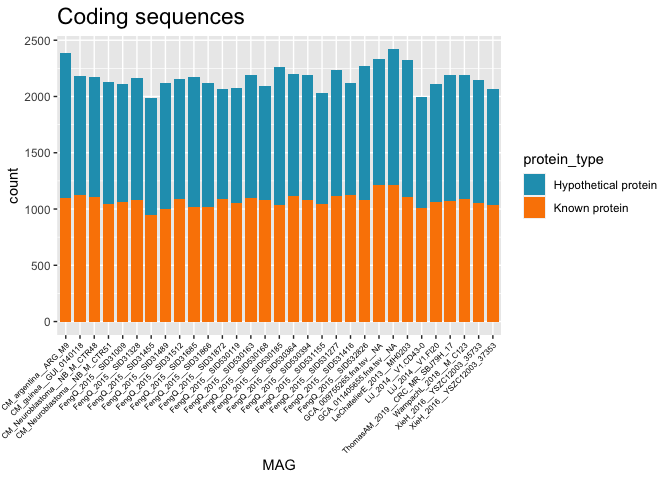
\includegraphics[width=0.7\textwidth]{prokka_data-1.png}
    \caption{\textbf{Number of coding sequences.} The number of coding sequences annotated for each MAG, divided in hypothetical and known proteins.}
    \label{fig:prokka1}
\end{subfigure}
\begin{subfigure}{0.49\textwidth}
    \centering
    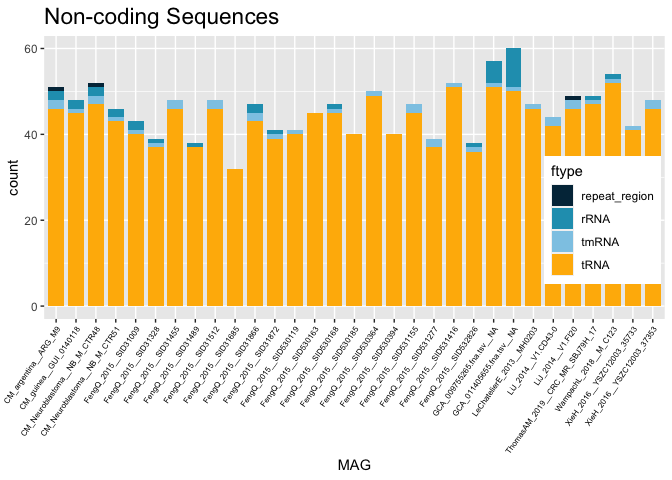
\includegraphics[width=0.7\textwidth]{prokka_data-2.png}
    \caption{\textbf{Number of non-coding sequences.} The number of non-coding sequences annotated for each MAG, divided in repeat regions, rRNAs, tmRNAs and tRNAs.}
    \label{fig:prokka2}
\end{subfigure}
\end{figure}

The number of CDS in the set of MAGs goes to a minimum of 1988 to a maximum of 2544. For each genome, about half of the CDSs are non-characterized hypothetical proteins(Fig. \ref{fig:prokka1}). For what concerns non-coding sequences, the vast majority of them is represented by tRNAs (Fig. \ref{fig:prokka2}).
\subsection*{Pangenome Analysis}
\graphicspath{{images/pangenomeAnalysis}}

% plots to be included:
% - conserved vs total genes




% Pangenome analysis:
% what’s the size of your pangenome? Is it closed or open?
% How many core and accessory genes?

Pangenome analysis found 4670 total genes (figure \ref{fig:pangenome pie}), 
among which 1017 were attributed to the \emph{core} (above 90\% prevalence in MAGs),
2074 to the \emph{shell} (from 15\% to 89\% prevalence), and 1579 were classified as \emph{cloud}
(from 0\% to 15\% prevalence). The results were robust with respect to many rounds of computation.

The number of conserved genes appears to reach a plateau (figure \ref{fig:conserved vs total})
when the number of MAGs increases, suggesting that this species has a closed pangenome.
This is further confermed by the trend of unique genes plotted against the number of
genomes (figure \ref{fig:unique vs new}).

The plot of pangenome frequencies ?? (figure \ref{fig:pangeome frequency}) shows the typical shape observed in microbiome samples.
It is U shaped since there are conserved functions (core genes) that are present in every strain, and
other genes that are very specific and are present in only one or few strains (unique genes), with very few genes in between.

\begin{figure}[h]	% to be fixed
     \centering
     \begin{subfigure}[b]{0.4\textwidth}
         \centering
         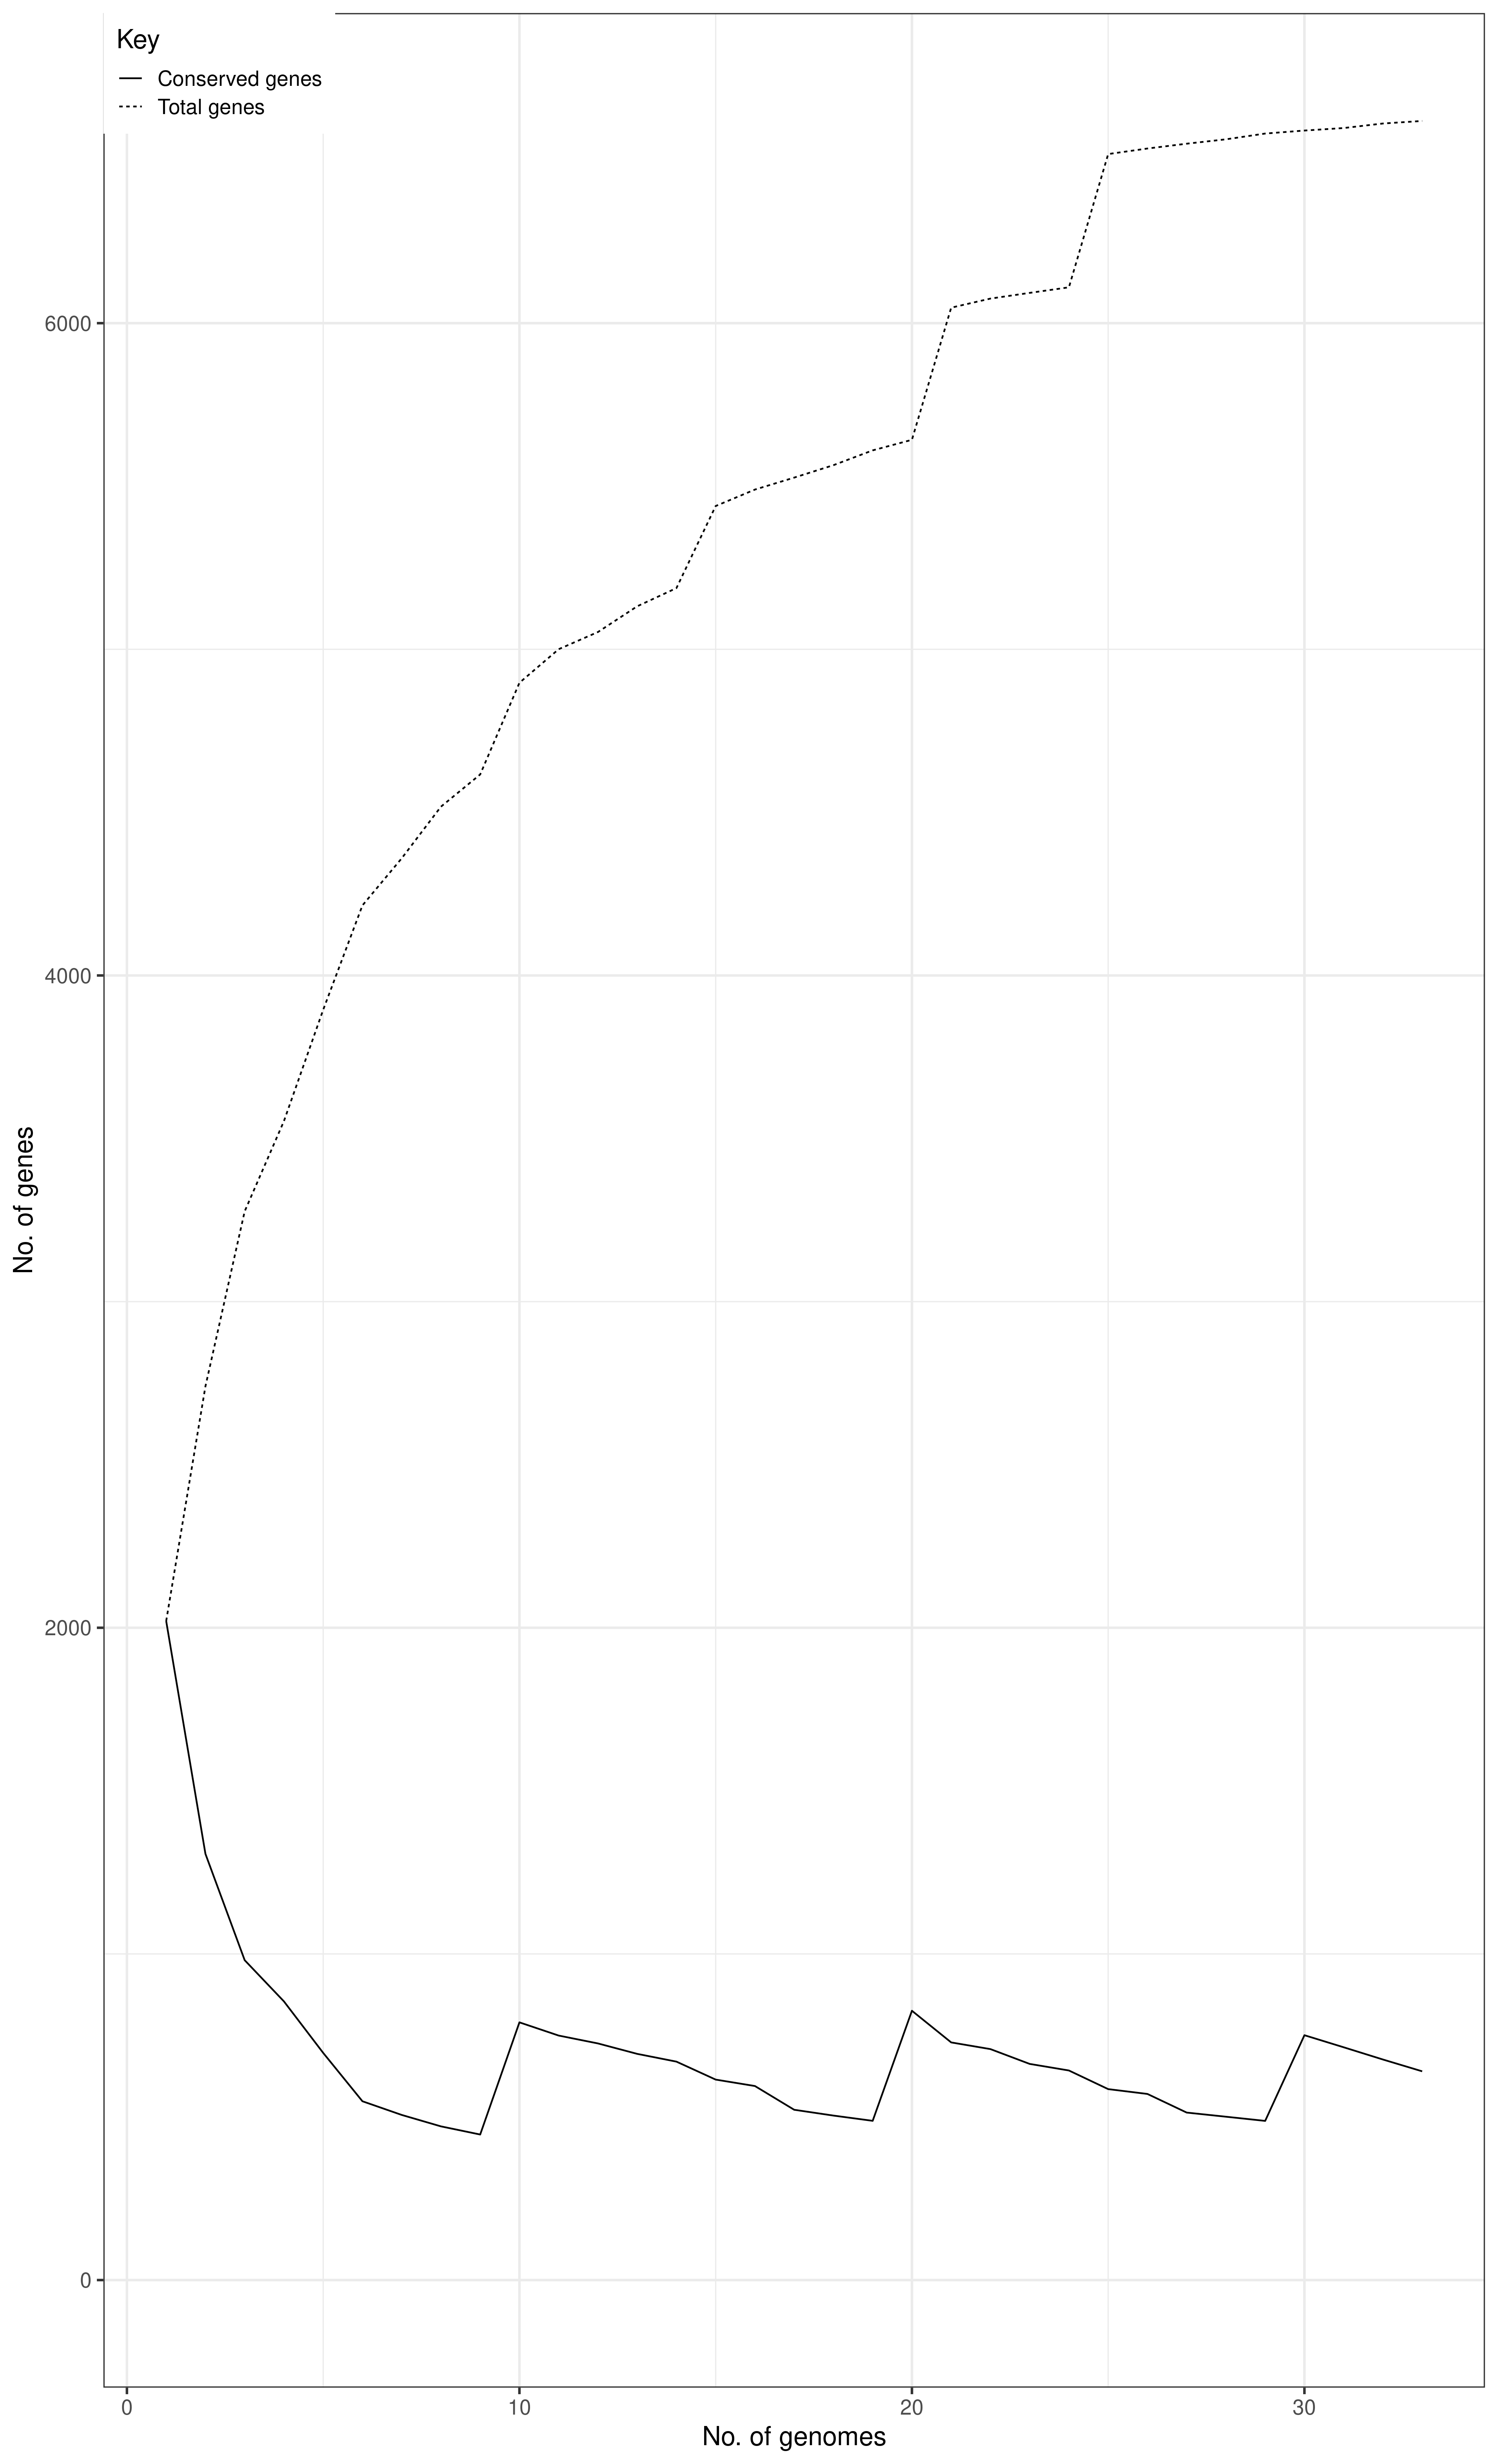
\includegraphics[width=\textwidth]{conserved_vs_total_genes}
         \caption{\scriptsize{The trend of conserved genes suggest that the species analyzed
                                has a closed pangenome}}
         \label{fig:conserved vs total}
     \end{subfigure}
     \hfill
     \begin{subfigure}[b]{0.4\textwidth}
         \centering
         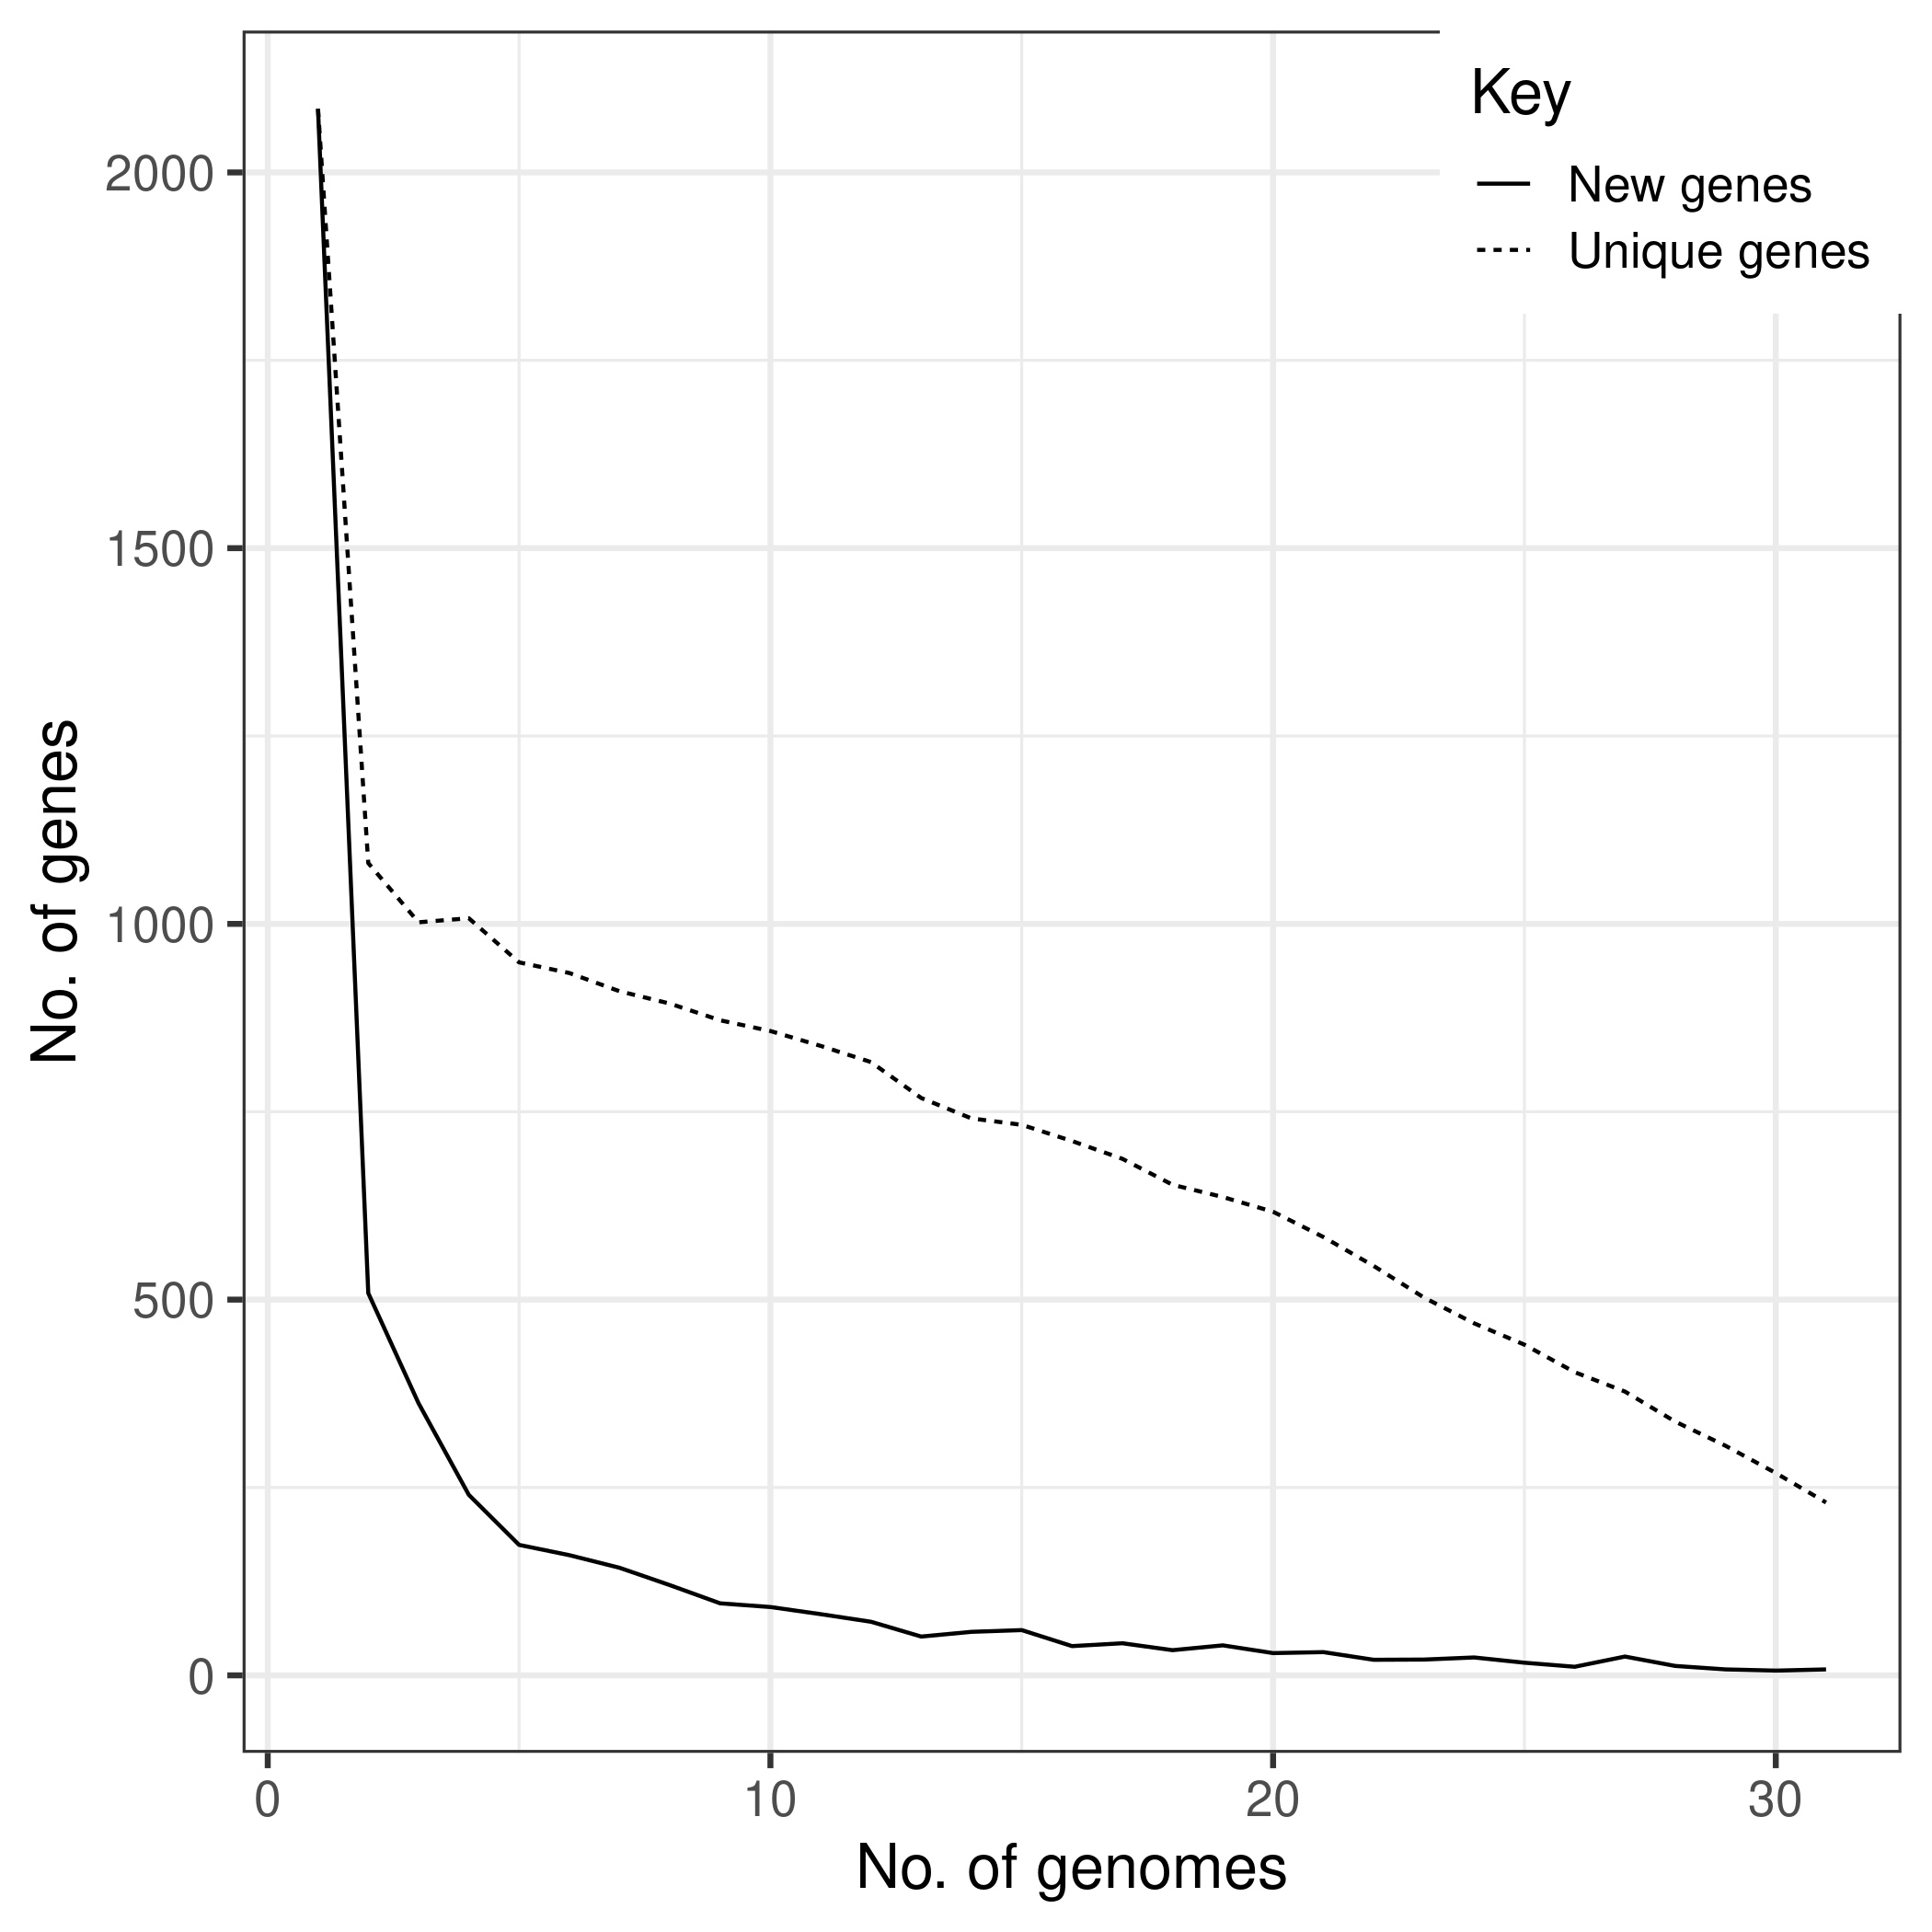
\includegraphics[width=\textwidth]{unique_vs_new_genes}
         \caption{}
         \label{fig:unique vs new}
     \end{subfigure}
        \caption{}
        \label{fig:conserved_unique_genes}
\end{figure}


\begin{figure}[h]	% to be fixed
     \centering
     \begin{subfigure}[b]{0.45\textwidth}
         \centering
         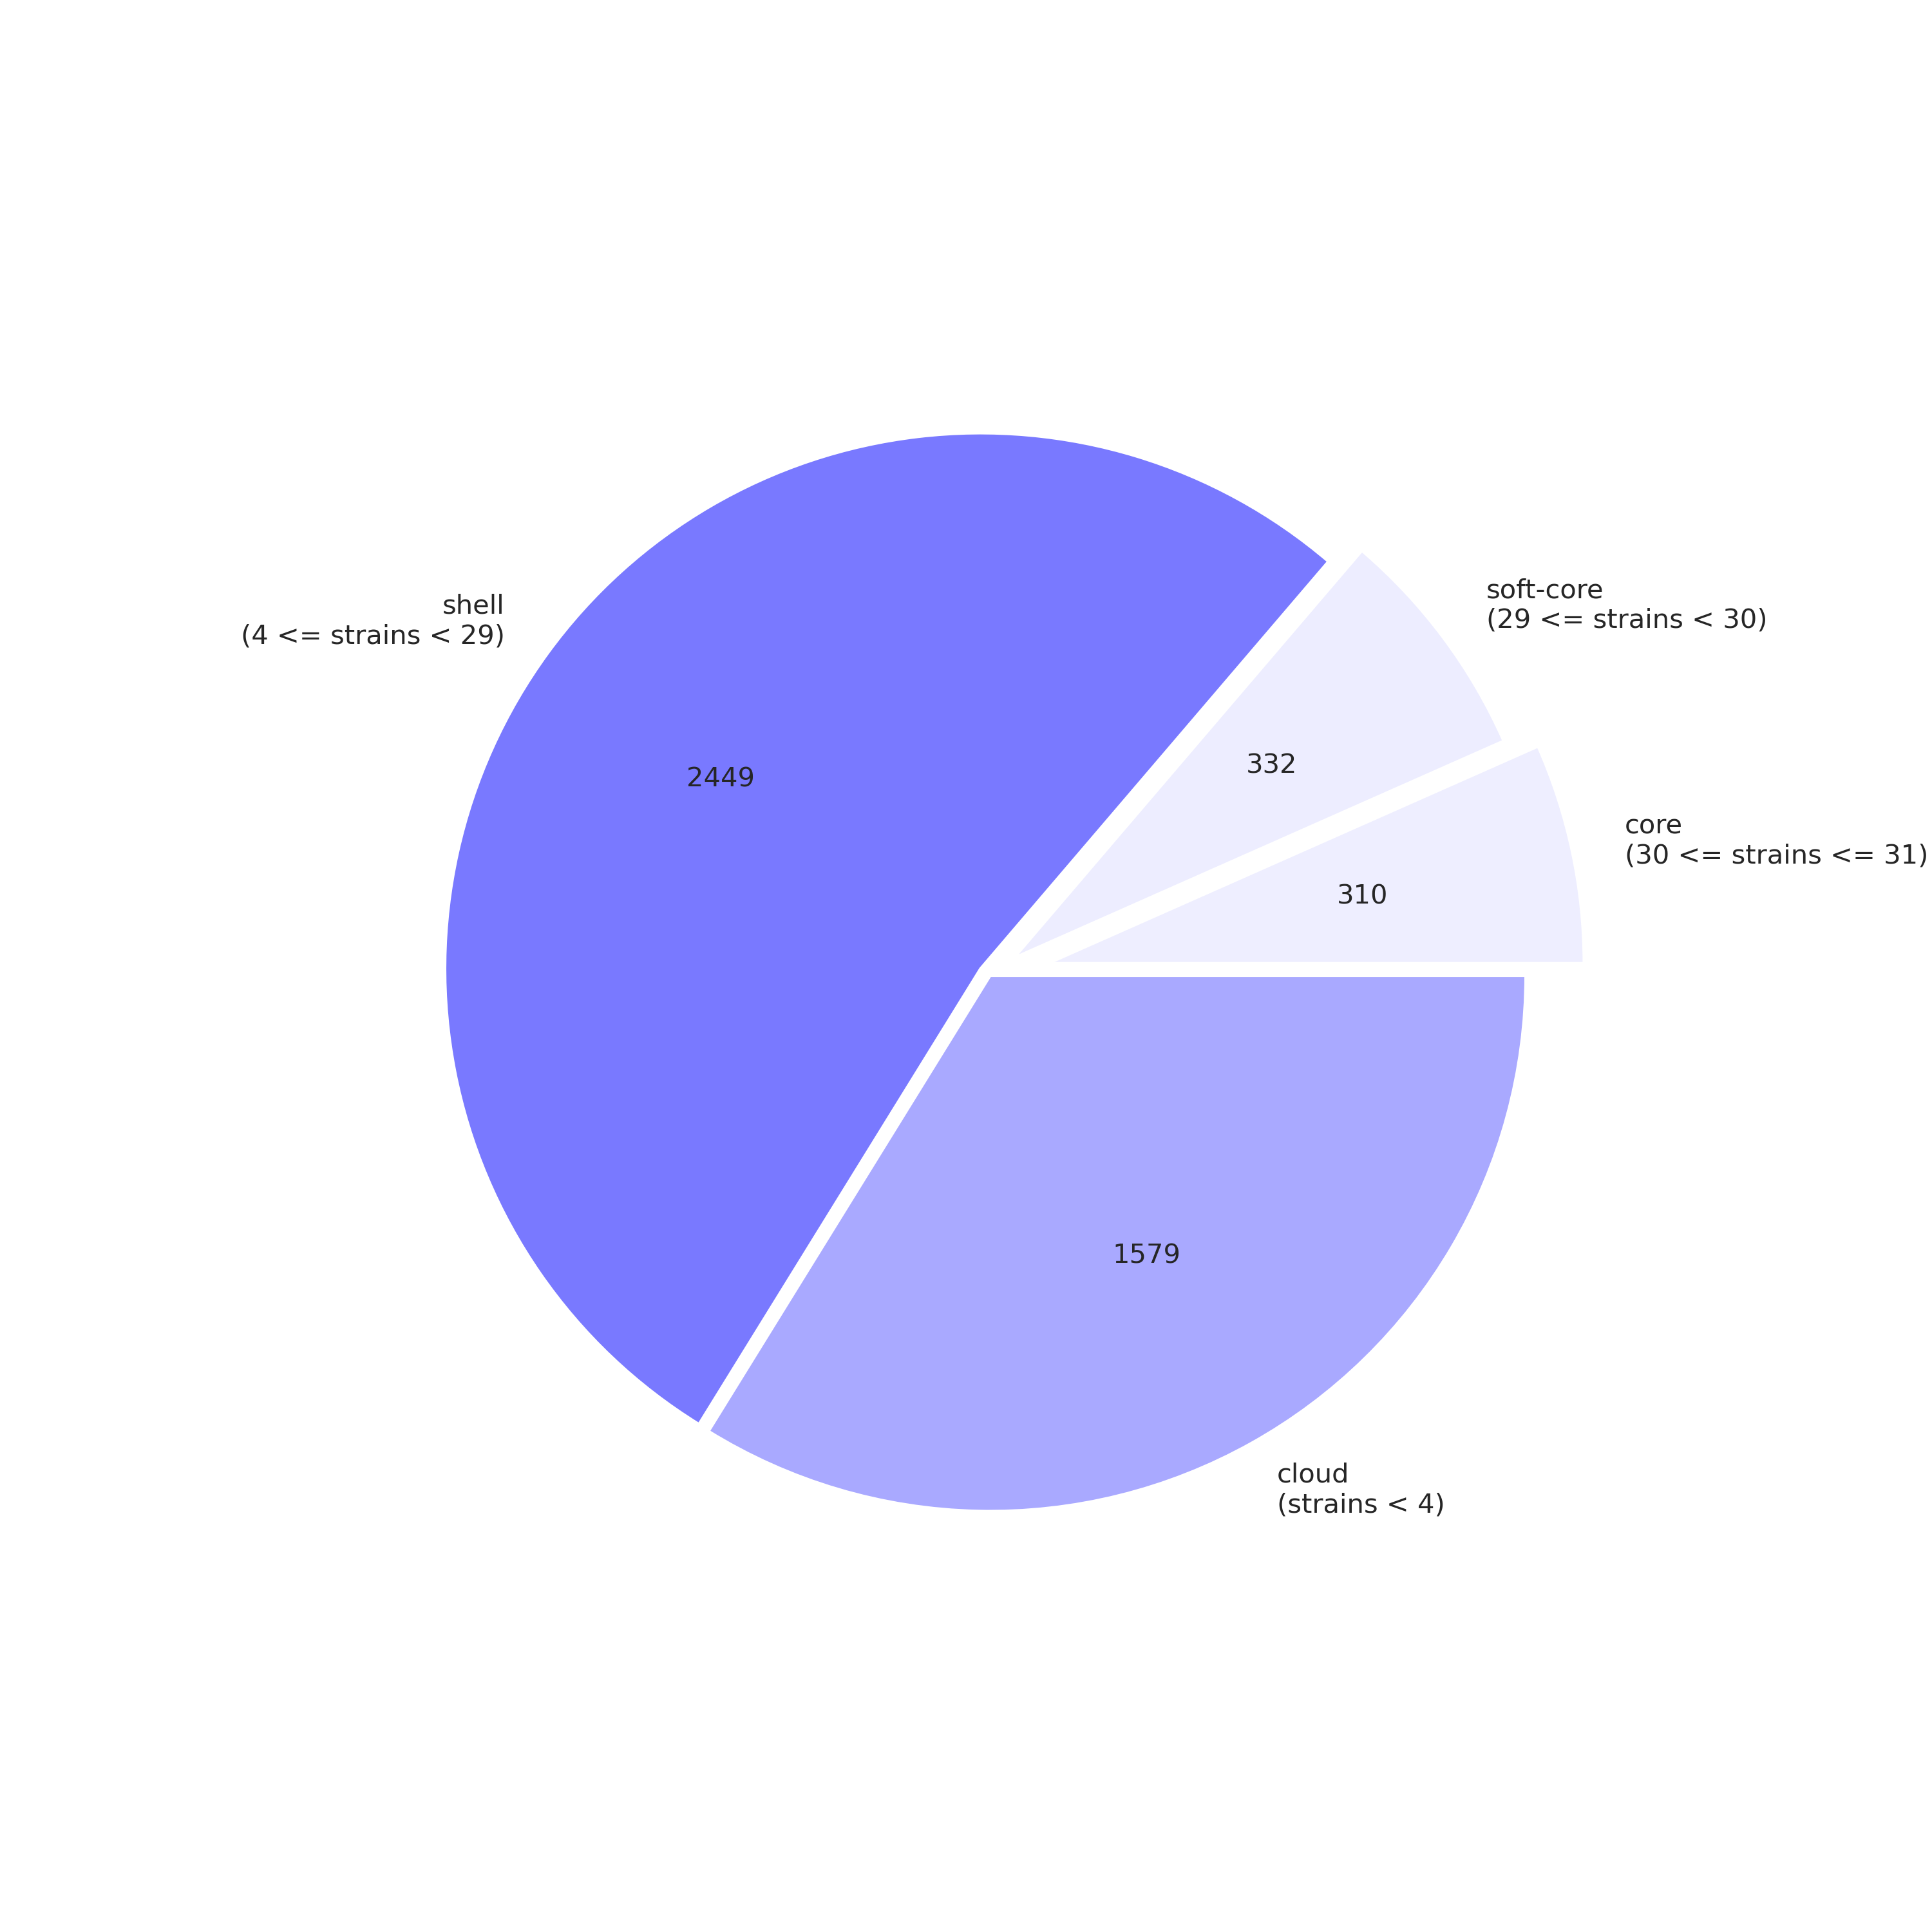
\includegraphics[width=\textwidth]{pangenome_pie}
         \caption{}
         \label{fig:pangenome pie}
     \end{subfigure}
     \hfill
     \begin{subfigure}[b]{0.45\textwidth}
         \centering
         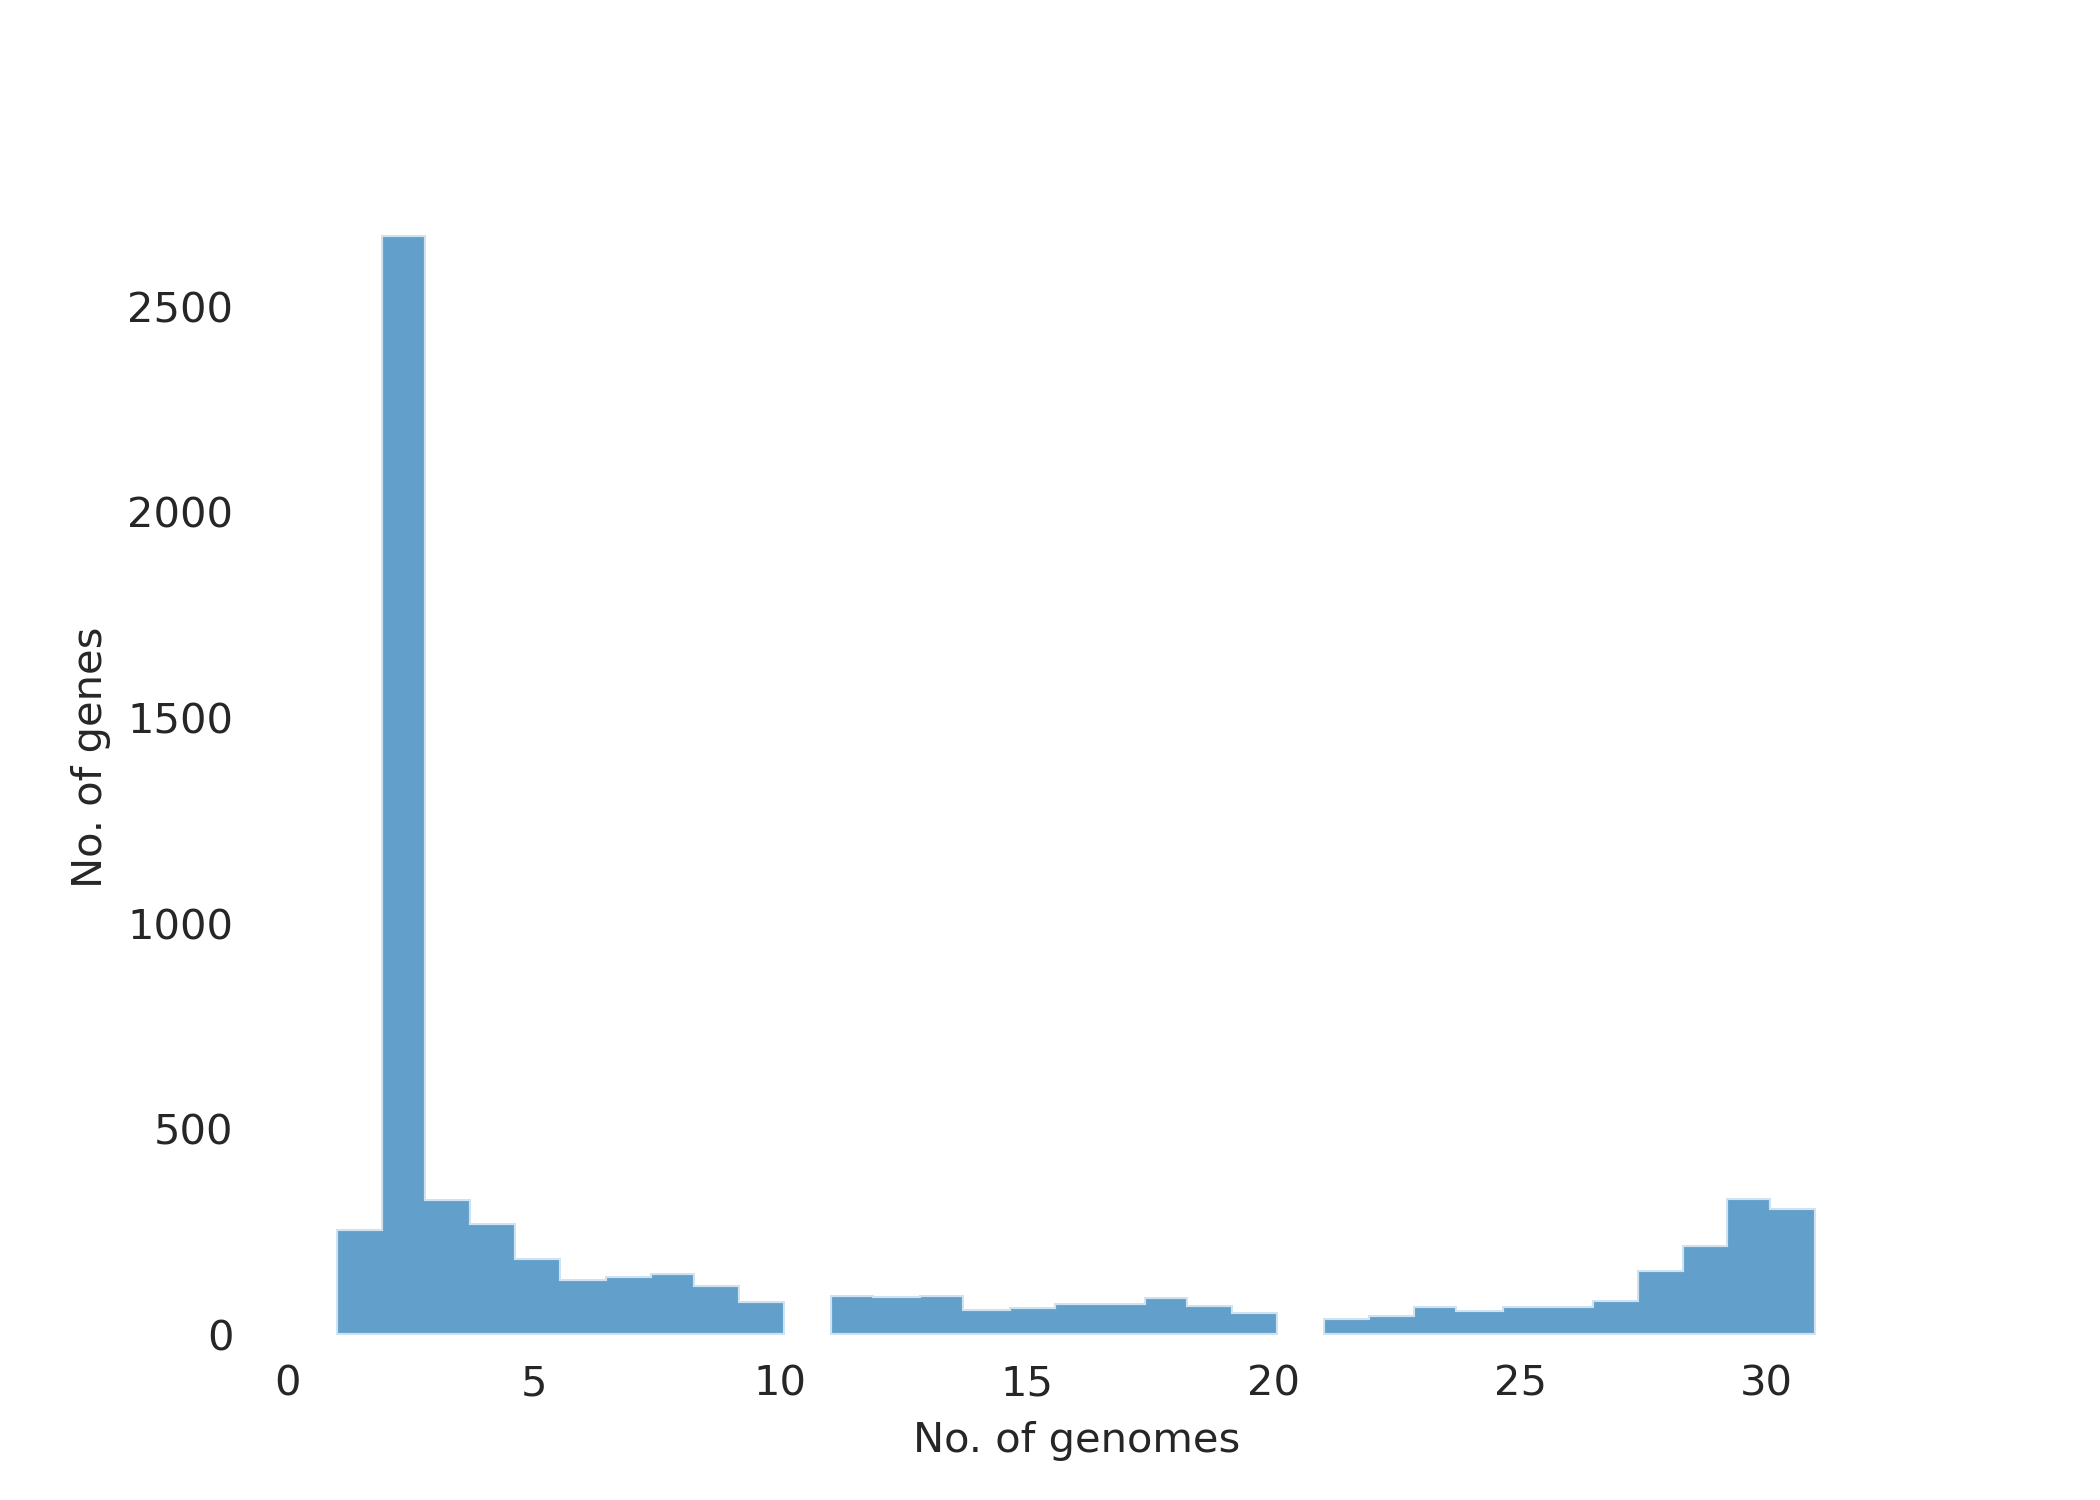
\includegraphics[width=\textwidth]{pangenome_frequency}
         \caption{}
         \label{fig:pangeome frequency}
     \end{subfigure}
     \hfill
     \begin{subfigure}[b]{0.85\textwidth}
         \centering
         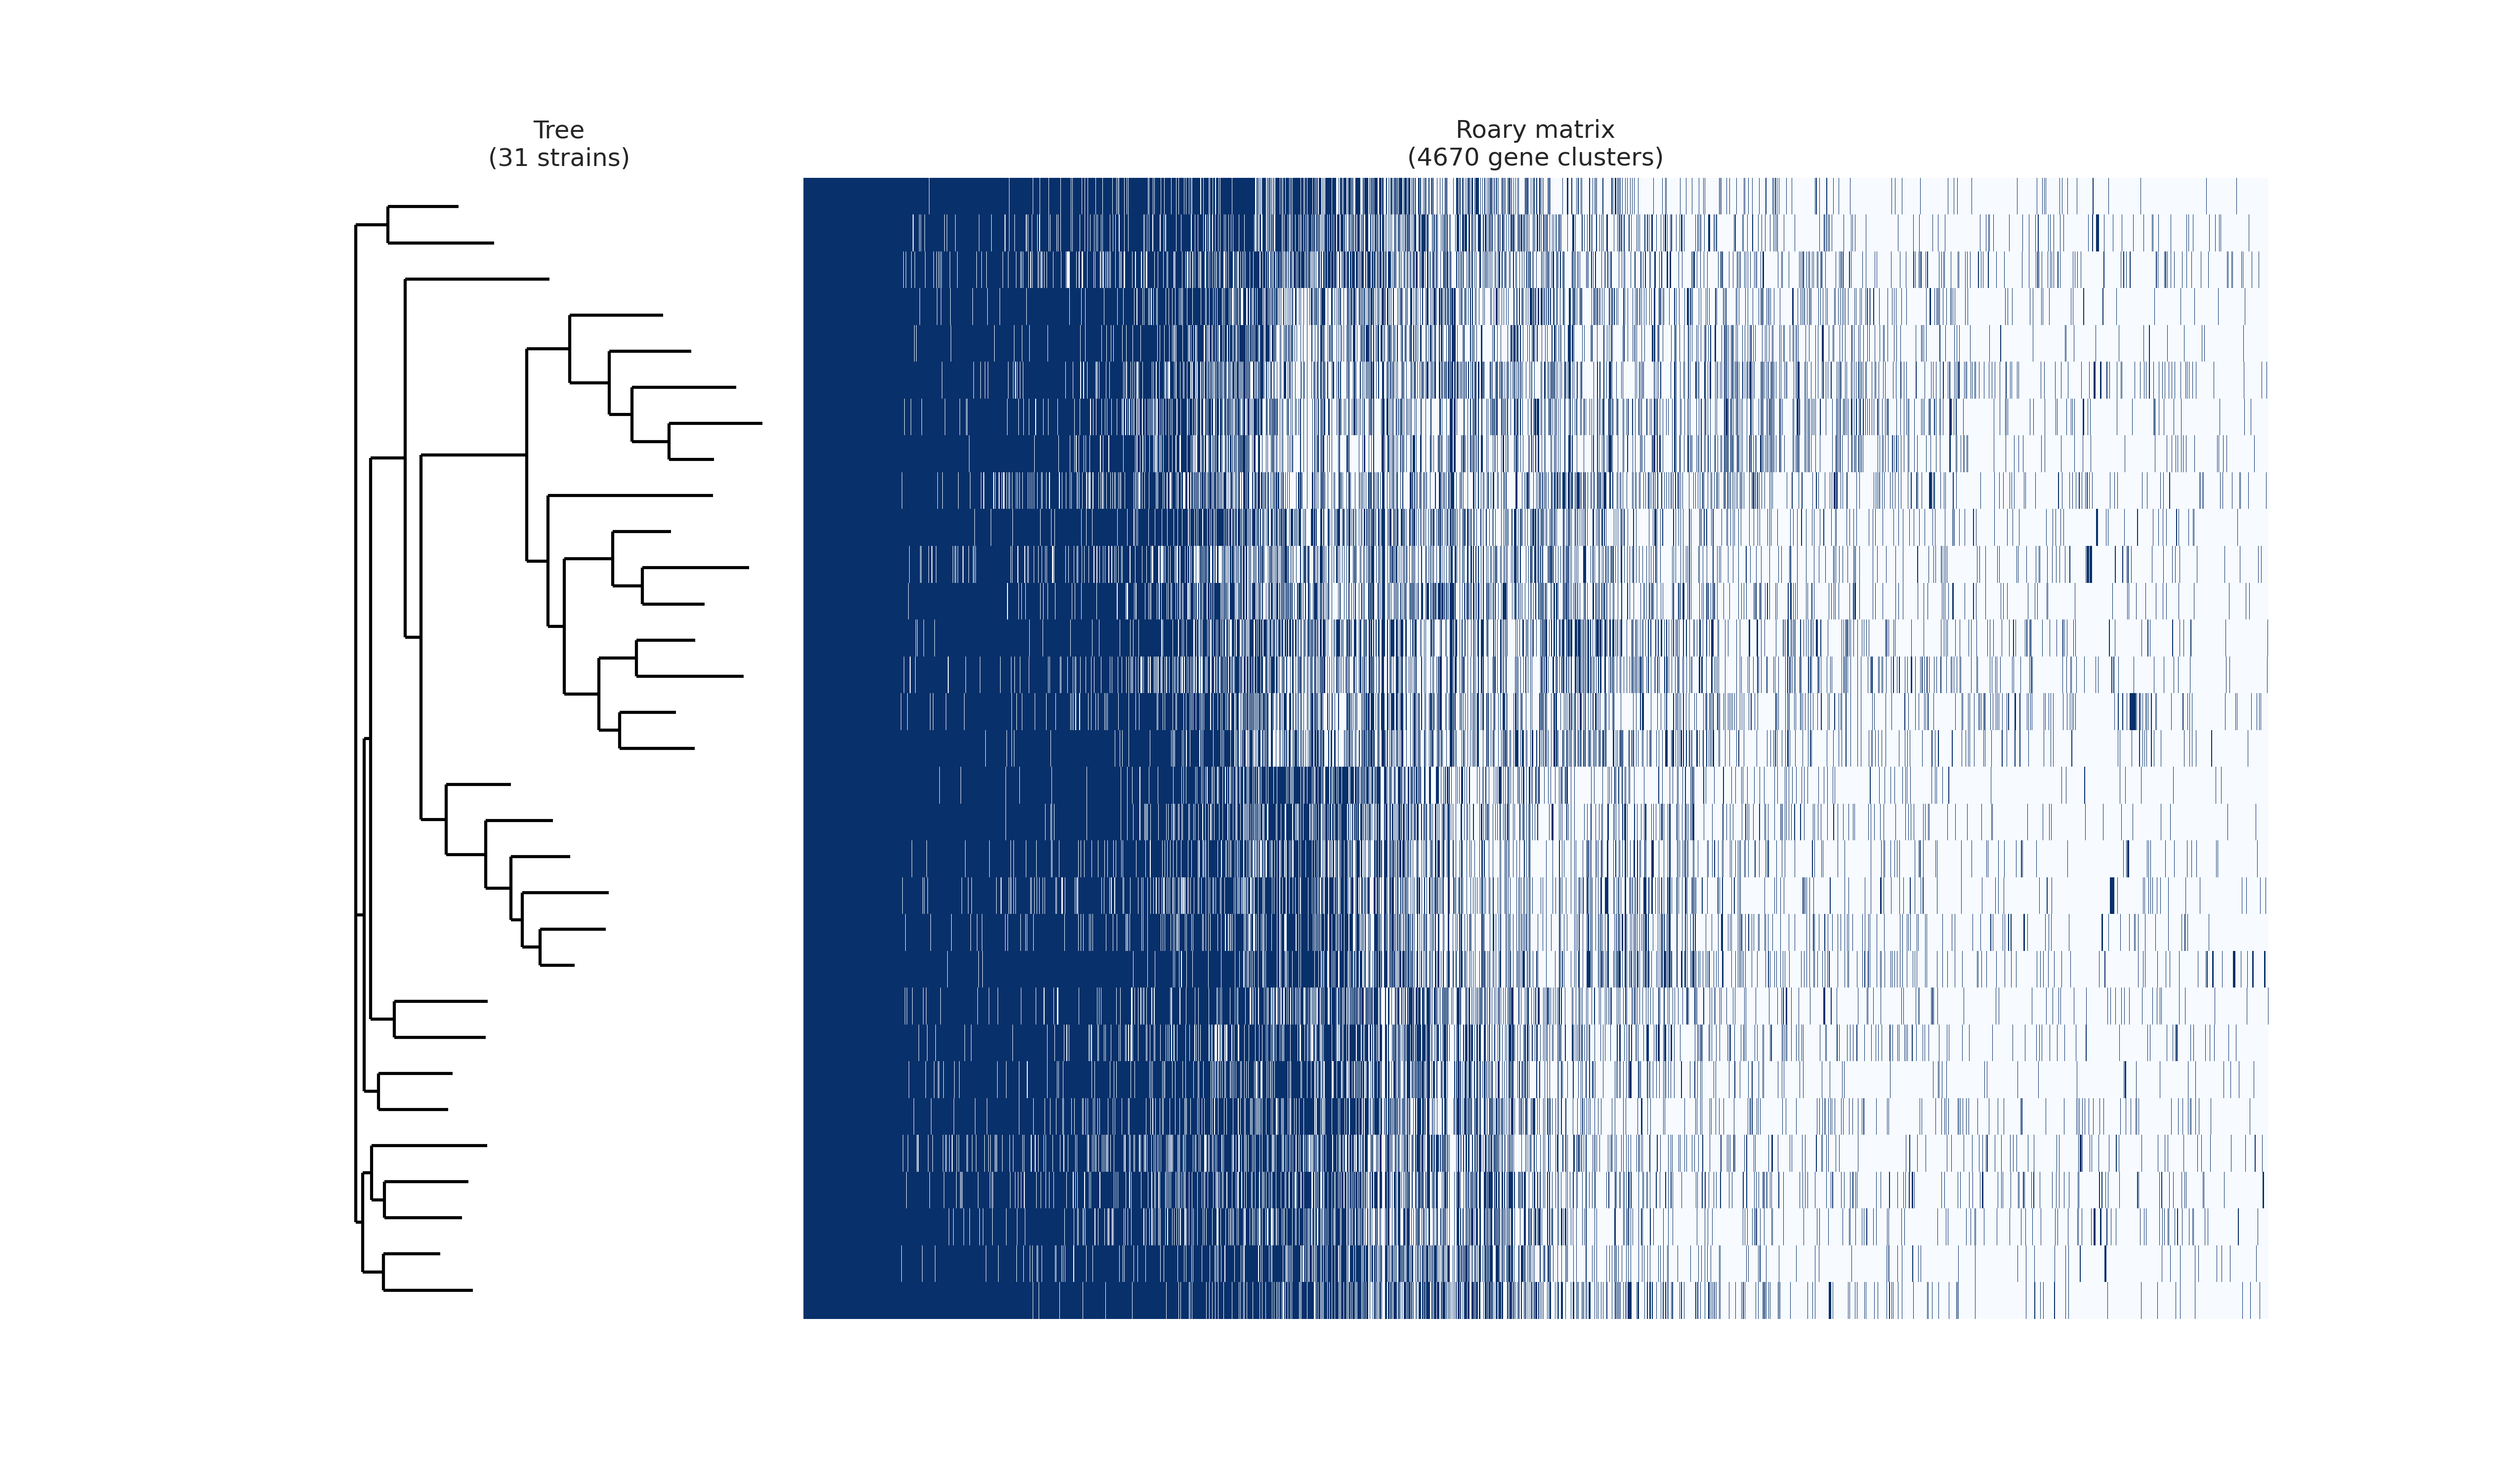
\includegraphics[width=\textwidth]{pangenome_matrix}
         \caption{}
         \label{fig:pangenome matrix}
     \end{subfigure}
        \caption{Three simple graphs}
        \label{fig:pangenome}
\end{figure}



% (https://github.com/sanger-pathogens/Roary/blob/master/bin/create_pan_genome_plots.R)
% 
% - Pangenome frequency plot
% - Presence and absence matrix and tree
% - Pangenome pie-chart (core, soft core, shell and cloud genes)
% (https://github.com/sanger-pathogens/Roary/blob/master/contrib/roary_plots/roary_plots.py)






















\subsection*{Phylogenetic Structure and association with host data}
\graphicspath{{images/phylogeneticStructureHostData/}}


% Phylogenetic analysis and association with host data: comparison of phylogenetic
% trees based on accessory gene presence/absence or on core gene alignment.
% Do you detect clusters of strains? How do they associate with the metadata?

Significant differences in the topology were found between the tree obtained from the presence/absence of accessory genes
and the one built from the core gene alignement (figure \ref{fig:phylogenetic trees}). Instead,
MAFFT and PRANK produced core gene alignements that resulted in identical trees
(figure \ref{core alignement mafft tree}). 

Three main clusters of strains were seen in the tree obtained from the alignement, but the low number of samples and the high fragmentation of
information seen in the metadata impede the observation of finer clustering. 
For instance, no clustering with respect to the country nor to the disease were visible.


\begin{figure}[h!]
    \centering
    \begin{subfigure}[b]{0.7\textwidth}
        \centering
        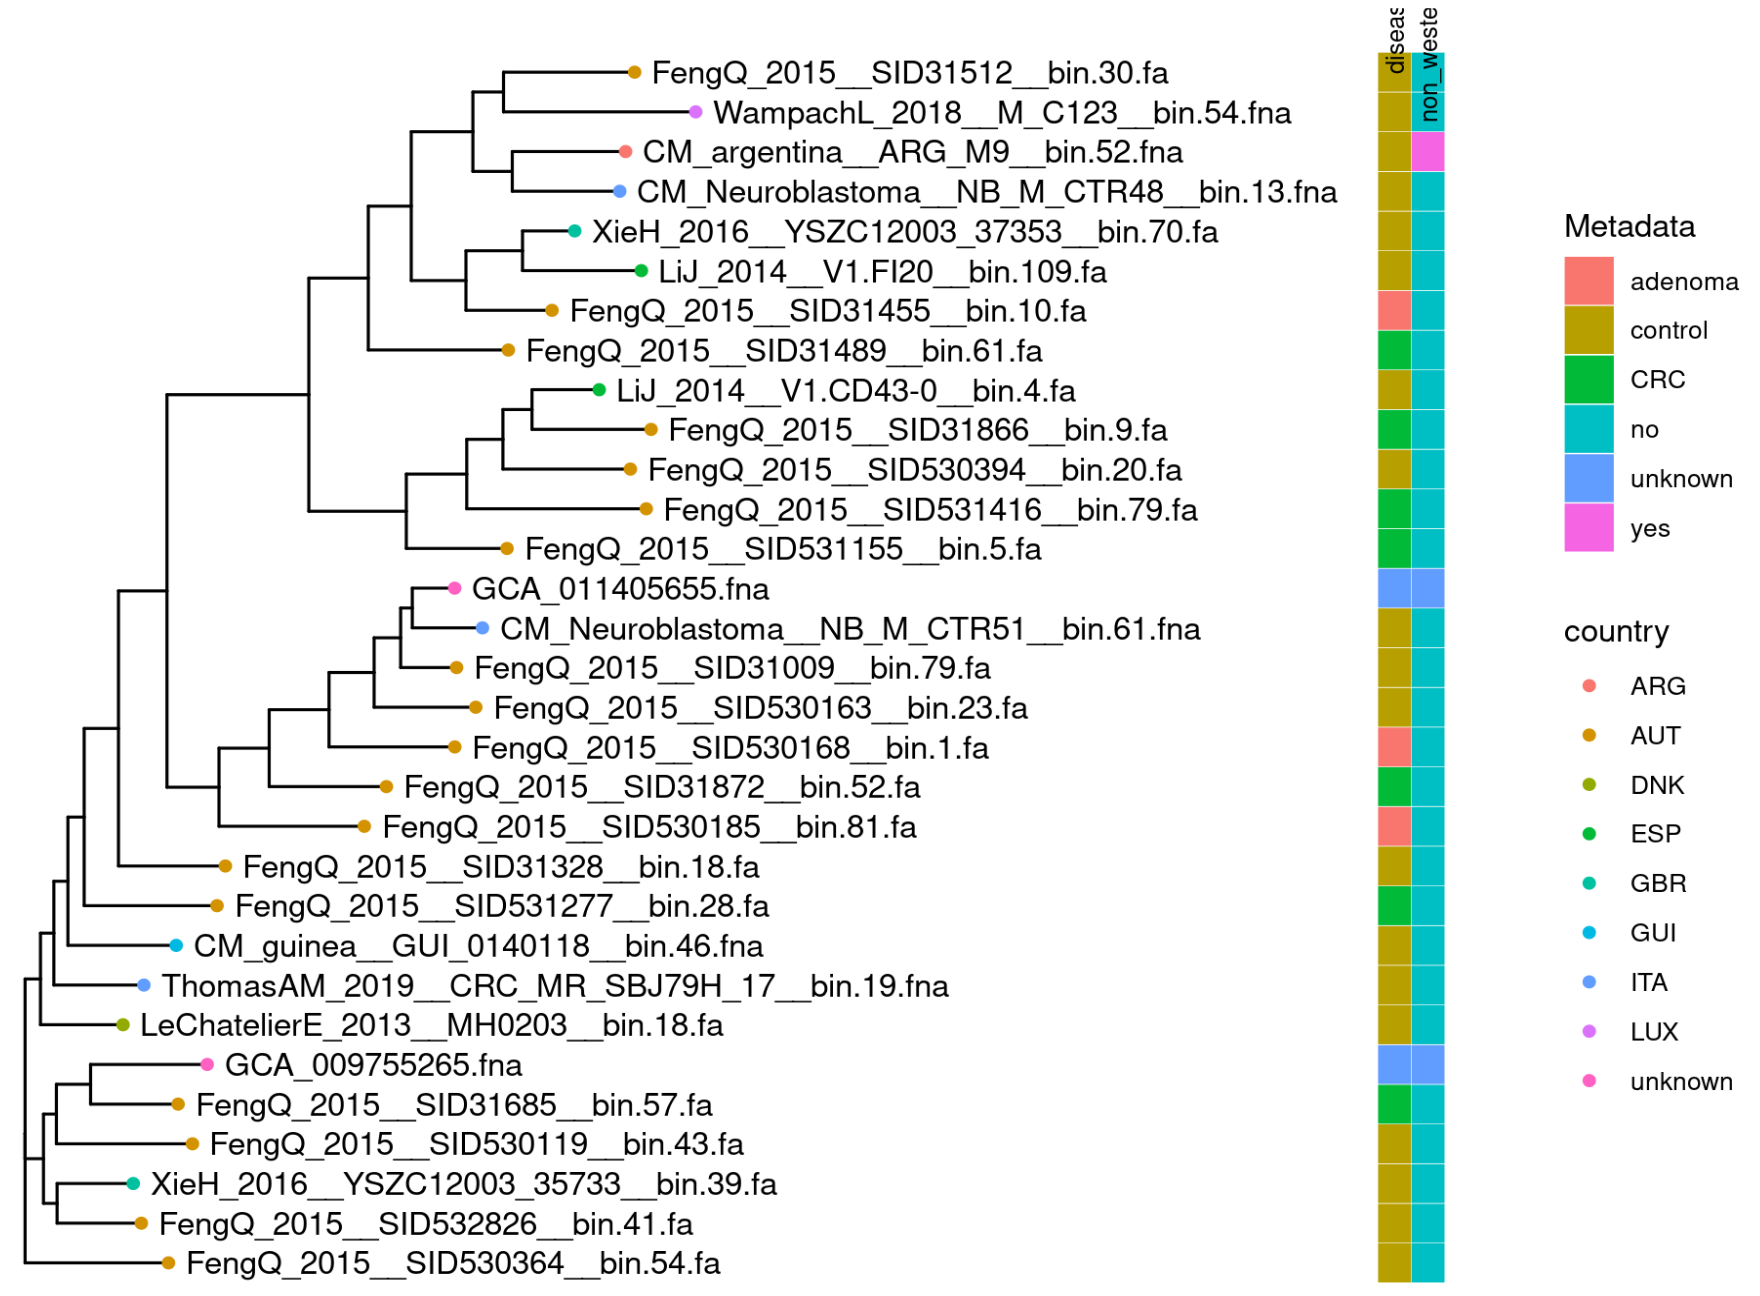
\includegraphics[width=\textwidth]{enriched_tree_prank_final.png}
        \caption{}
        \label{fig:core alignment prank tree}
    \end{subfigure}
    \begin{subfigure}[b]{0.7\textwidth}
        \centering
        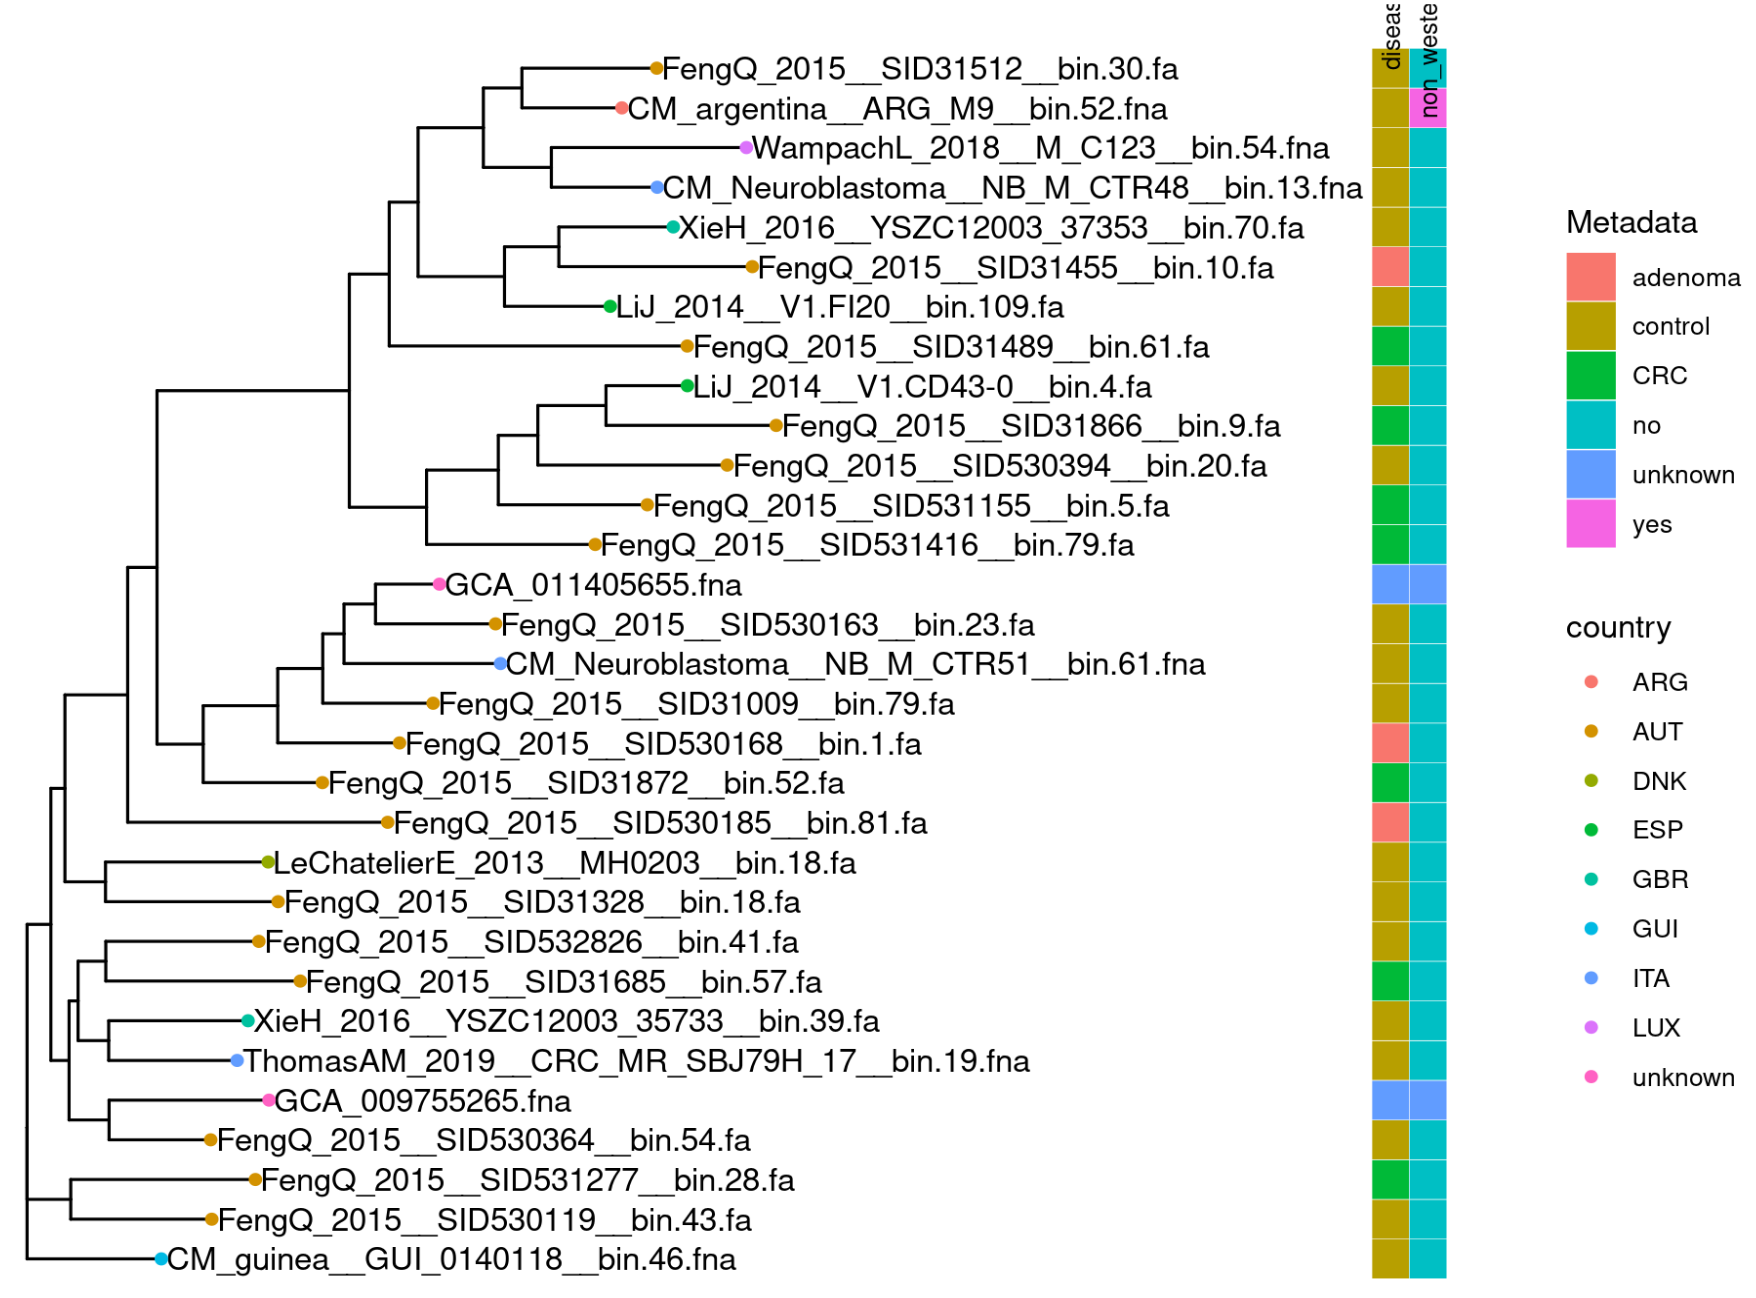
\includegraphics[width=\textwidth]{enriched_tree_Newick_final.png}
        \caption{}
        \label{fig:presence absence tree}
    \end{subfigure}
       \caption{}
       \label{fig:phylogenetic trees}
\end{figure}







\clearpage
\section*{Conclusion}

In this study, 31 high quality genomes (29 MAGs and 2 reference genomes)
of the organism \emph{Adlercreutzia equolifaciens} were characterized.
The set of MAGs was derived from a pool of individuals that was heterogeneous
with respect to country of provenence, health status, diseases, and age. 

All the strains were correctly classified to the species. 
Genome annotation was performed to retrieve informations about the genomes, that 
were used to perform pangenome analysis, trough which the pangenome was found to be closed.

Subsequently, the phylogenetic structure was computed, and, considering the host metadata,
no significant clusters were found between the strains. As expected, the phylogeny 
retrieved from the presence or absence of accessory genes perfomed diffently with respect
to the one obtained from the core gene alignement, with the last one to be considered
more reliable. 










\clearpage
\appendix
\section*{Supplementary data}
\graphicspath{{images/pangenomeAnalysis/}}


\begin{figure} 
     \centering
     \begin{subfigure}[b]{0.45\textwidth}
         \centering
         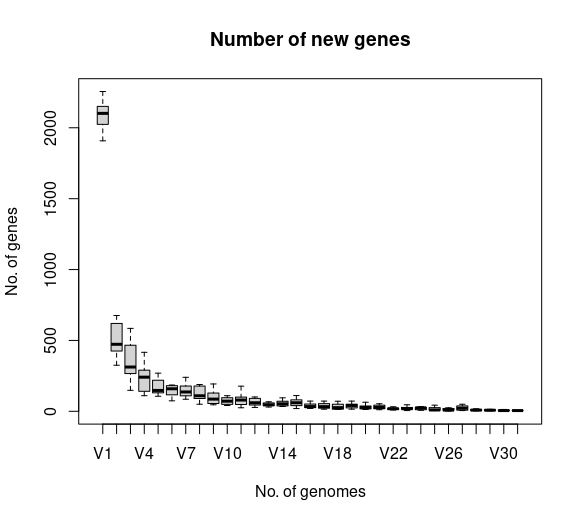
\includegraphics[width=\textwidth]{number_new_genes}
         \caption{Number of new genes}
         \label{fig:new genes}
     \end{subfigure}
     \hfill
     \begin{subfigure}[b]{0.45\textwidth}
         \centering
         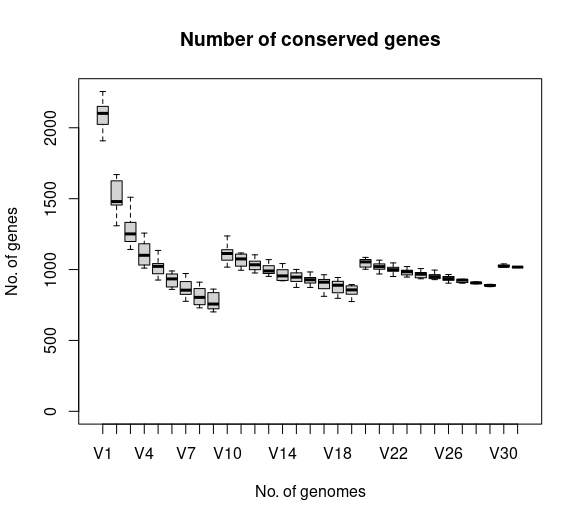
\includegraphics[width=\textwidth]{number_conserved_genes}
         \caption{Number of conserved genes}
         \label{fig:conserved genes}
     \end{subfigure}
     \hfill
     \begin{subfigure}[b]{0.45\textwidth}
         \centering
         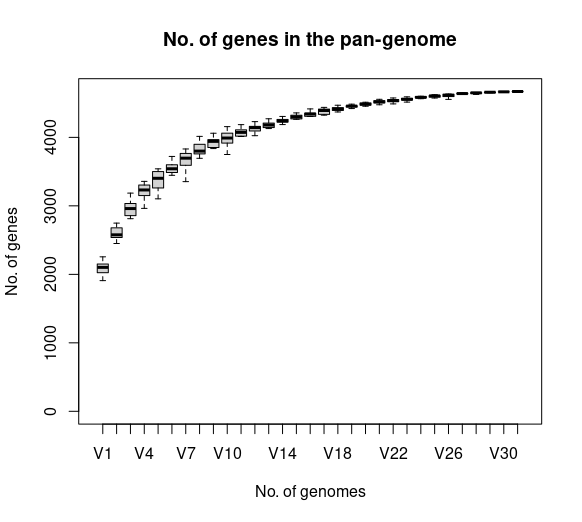
\includegraphics[width=\textwidth]{number_genes_pangenome}
         \caption{Number of genes in the pan-genome}
         \label{fig:pagenome genes}
     \end{subfigure}
     \hfill
     \begin{subfigure}[b]{0.45\textwidth}
         \centering
         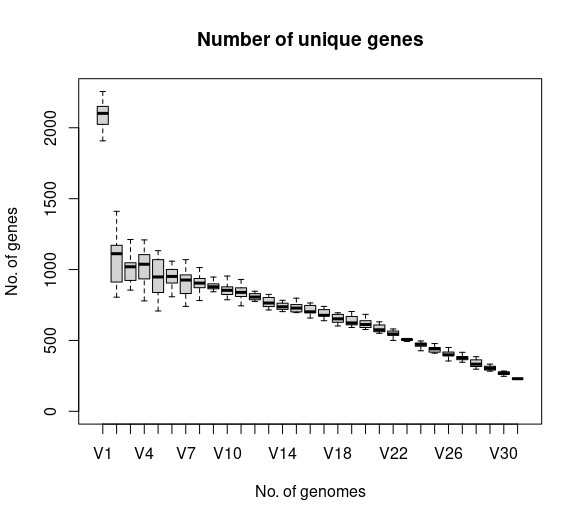
\includegraphics[width=\textwidth]{number_unique_genes}
         \caption{Number of unique genes}
         \label{fig:pagenome genes}
     \end{subfigure}
     \hfill
     \begin{subfigure}[b]{0.45\textwidth}
         \centering
         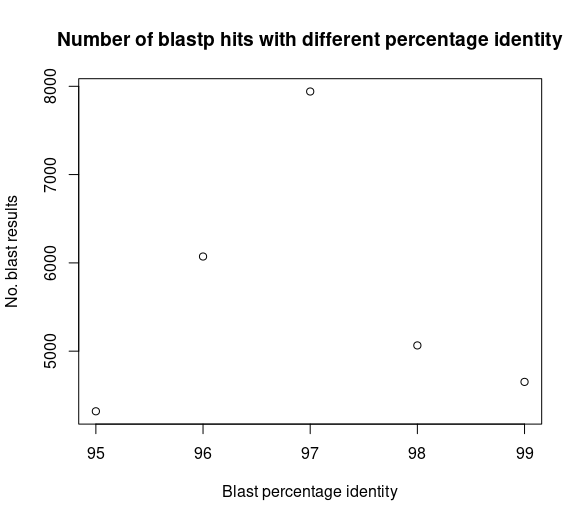
\includegraphics[width=\textwidth]{number_blastp_hits_diff_identity}
         \caption{Number of blastp hits with different percentage identity}
         \label{fig:blastp identity}
     \end{subfigure}
        \caption{Three simple graphs}
        \label{fig:genes vs genomes}
\end{figure}




\clearpage
\printbibliography

\end{document}
